\chapter{Realizability}
\label{chap:realizability}

\section{Motivation}
\label{sec:realizability-basic-idea}

Realizability was introduced by Stephen Kleene~\sidecite{KleeneSC:intint} who used it to build a model of intuitionistic arithmetic. We motivate it by asking a practical question: given a mathematical structure (a set equipped with operations and relations satisfying some axioms), what should its implementation look like?

For simple cases, the answer is obvious. A group is implemented by a type whose values represent its elements, a value
representing the neutral element, and functions which compute the group operation and inverses.
But for more interesting structures, especially those arising in mathematical analysis, the answer is less clear. How do we implement the real numbers? Which operations on a compact metric space can be implemented? How do we implement a space of smooth functions? Significant research goes into finding satisfactory answers to such questions~\sidecite{Wei00,TZ98,Bla97}.

To explain the basic idea behind realizability we consider a small real-world programming example. Suppose we are asked to design a data structure for the set $\mathsf{Graphs}$ of all finite simple\sidenote{A graph is \defemph{simple} when there is at most one edge between any two vertices.} directed graphs with vertices labeled by distinct integers, such at the graph $G$ shown below:
%
\begin{center}
  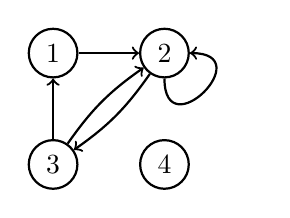
\begin{tikzpicture}
    \node [circle, thick, draw] at ( 45 : 1) (B) {2} ;
    \node [circle, thick, draw] at (135 : 1) (A) {1} ;
    \node [circle, thick, draw] at (225 : 1) (C) {3} ;
    \node [circle, thick, draw] at (315 : 1) (D) {4} ;
    \draw[thick,->] (A) -- (B) ;
    \draw[thick,->] (B) edge [in=0, out=270, looseness=5] (B) ;
    \draw[thick,->] (B) edge [bend left=10] (C) ;
    \draw[thick,->] (C) -- (A) ;
    \draw[thick,->] (C) edge [bend left=10] (B) ;
  \end{tikzpicture}
\end{center}
%
A common representation of graphs uses a pair of lists $(\ell_V, \ell_A)$, where $\ell_V$ is the list of vertex labels and $\ell_A$ the \emph{adjacency list} representing the arrows as pairs of labels. For the above graph these would be $\ell_V = [1, 2, 3, 4]$ and $\ell_A = [(1,2), (2,2), (2,3), (3,2), (3,1)]$.
%
Thus we define the datatype of graphs as\sidenote{We use Haskell notation in which $[t]$ is the type of lists of
  elements of type~$t$, and $(t_1, t_2)$ is the cartesian product of types~$t_1$ and~$t_2$.}
%
\begin{lstlisting}[language=Haskell]
type Graph = ([Int], [(Int, Int)])
\end{lstlisting}
%
However, this is not a complete description of the intended representation, as there are representation invariants and conditions not expressed by the type:
%
\begin{itemize}
\item the order in which the vertices and arrows are listed is not
  important,
\item each vertex and arrow must be listed exactly once, and
\item the source and target of each arrow must appear in the list of vertices.
\end{itemize}
%
A complete implementation of $\mathsf{Graphs}$ must not only specify the underlying
datatype $\mathtt{graph}$, but also relate its values to the elements of~$\mathsf{Graphs}$, which can be expressed with a \defemph{realizability relation}
%
\begin{equation*}
  r \rz x
\end{equation*}
%
read as ``datum~$r$ realizes (implements, represents) element~$x$''. In the above example we would write
%
\begin{equation*}
([1, 2, 3, 4], [(1,2), (2,2), (2,3), (3,2), (3,1)]) \rz G,
\end{equation*}
%
and also
%
\begin{equation*}
([3, 2, 1, 4], [(2,2), (1,2), (2,3), (3,2), (3,1)]) \rz G.
\end{equation*}
%
Once the set $\mathsf{Graphs}$ is implemented as a datatype, we would like to compute with it.
%
Programmers know what it means to implement, or realize, a map $f : \mathsf{Graphs} \to \mathsf{Graphs}$, namely to give a program $p : \mathtt{graph} \to \mathtt{graph}$ which does to realizers what~$f$ does to elements: if $r \rz G$ then $p \, r \rz f(G)$. We say that~$f$ is \defemph{realized} or \defemph{tracked} by~$p$.

\section{Assemblies}
\label{sec:assemblies}

We now give a precise definition of the ideas presented in the previous section.

\begin{definition}
  Let $\AA$ be a tpca and $\subAA$ a sub-tpca. An \defemph{assembly} over~$(\AA, \subAA)$ is a triple
  $\asm{S} = \xasm{S}$ where $S$ is a set, $|S|$ is a type, and $\rz_S$ is a relation between $\xAtyp{S}$ and~$S$
  satisfying: for every $x \in S$ there is $\R{x} \in \xAtyp{S}$ such that $\R{x} \rz_S x$.

  An \defemph{assembly map} $f : \asm{S} \to \asm{T}$ between assemblies $\asm{S}$ and $\asm{T}$ is a map $f : S \to T$
  between the underlying sets for which there exists $\R{f} \in \compAtyp{|S| \to |T|}$, called a \defemph{realizer}
  of~$f$, satisfying: if $\R{x} \rz_S x$ then $\defined{\R{f} \, \R{x}}$ and $\R{f} \, \R{x} \rz_T f(x)$.
\end{definition}

We adopt the notational convention that a realizer for an element or a function is denoted by the same letter in
fixed-width font. Thus realizers for $x$, $y$, $f$, $g$ are denoted by $\R{x}$, $\R{y}$, $\R{f}$, $\R{g}$, respectively.

There are many versions of realizability. Ours is known as \defemph{typed relative realizability}. It is \emph{typed}
because we used typed pcas. It is \emph{relative} because maps are realized relative to a choice of a sub-pca. In
typical cases, such as type~2 machines and the graph model from \cref{sec:type-2,sec:graph-model}, $\subAA$ is the
computable part of~$\AA$. Thus relative realizability formalizes the slogan
%
\begin{center}
  \emph{``Continuous data -- computable functions!''}
\end{center}

When $\subAA = \AA$ we write $\Asm{\AA}$ instead of $\Asm{\AA,\AA}$.

When $\AA$ is untyped the definition of an assembly simplifies a bit because we need mention the (trivial) types.

\begin{definition}
  An \defemph{assembly} over an untyped pca~$\AA$ is a pair $\asm{S} = (S, {\rz_S})$ where $S$ is a set and $\rz_S$ is a relation between~$\AA$ and~$S$, such that for every $x \in S$ there is $r \in A$ and $r \rz_S x$.
\end{definition}

Assemblies and maps over $(\AA, \subAA)$ form a \defemph{category $\AsmA$}.
%
Indeed, if $f : \asm{S} \to \asm{T}$ and $g : \asm{T} \to \asm{U}$ are realized by $\R{f} \in \compAtyp{|S| \to |T|}$
and $\R{g} \in \compAtyp{|T| \to |U|}$, respectively, then their composition $g \circ f$ is realized by
$\tpcalam{x}{|S|}{r\,(q\,x)} = \combS\,(\combK\,r)\,(\combS\,(\combK\,q)\,(\combS\,\combK\,\combK))$.
%
The identity map $\id[S] : \asm{S} \to \asm{S}$ is realized by $\tpcalam{x}{|S|}{x} = \combS\,\combK\,\combK$. 
%
Composition is associative because it is just composition of maps.


\section{Modest sets}
\label{sec:modest-sets}

In the definition of assemblies, nothing prevents several elements from sharing a common realizer. We sometimes want
to prohibit such anomalies.

\begin{definition}
  An assembly $\asm{S}$ is \defemph{modest} when each $r \in \xAtyp{S}$
  realizes at most one element of~$S$. A modest assembly is also
  called a \defemph{modest set}.
\end{definition}

\noindent
In symbols, modesty\sidenote{The terminology ``modest'' was suggested by Dana Scott. It refers to the fact that the cardinality of a modest~$S$ set does not exceed the cardinality of $\xAtyp{S}$.} is the property
%
\begin{equation*}
  \all{r}{\xAtyp{S}}{
    \all{x,y \in S}
      (r \rz_S x \land r \rz_S y \implies x = y)
  }.
\end{equation*}
%
We let $\ModA$ be the full subcategory of $\AsmA$ on the modest sets is.

Most structures in computable mathematics turn out to be modest. However, sometimes assemblies are needed, and they form a slightly nicer category than the modest sets.

\section{Examples of assemblies}
\label{sec:examples-assemblies}


\subsection{Natural numbers}
\label{sec:asm-natural-numbers}


\subsection{Real numbers}
\label{sec:asm-real-numbers}


\subsection{Constant assemblies}
\label{sec:nabla}

The extreme case of elements sharing the same realizer happens when
all elements of a set share all realizers. Assemblies with this
property are called \defemph{constant assemblies}. They give us a way of
representing arbitrary sets.

Let $t$ be a type such that $\Atyp{t}$ is inhabited. Such a type
always exists, because there is at least one type $s$, and then
$\Atyp{s \to s \to s}$ contains $\combK_{s,s}$. Given any set $X$, let
$\nabla X = (X, t, {\rz_{\nabla X}})$ be the assembly whose underlying
set is~$X$ and the realizability relation is trivial, i.e., $r
\rz_{\nabla X} x$ for all $x \in X$ and $r \in A_t$. If $f : X \to Y$
is any map between sets~$X$ and~$Y$ then~$f$ is a morphism $\nabla f :
\nabla X \to \nabla Y$ because it is tracked by
$\tpcalam{x}{t}{x}$. This defines a functor
%
\begin{equation*}
  \nabla : \Set \to \AsmA.
\end{equation*}
%
Up to natural isomorphism, $\nabla$ is independent of the choice of
type~$t$. We will study the properties of $\nabla$ later on. For now
we notice that $\nabla$ is full and faithful, which means that
$\AsmA$ contains the category of sets as a full
subcategory.

The functor $\nabla$ is devoid of any computational content because it
represents a set~$X$ by a trivial realizability relation which conveys
no information at all about the elements of~$X$. Consequently, from
the realizers we cannot compute anything interesting regarding~$X$.

\begin{exercise}
  Let $\Gamma : \AsmA \to \Set$ be the forgetful functor which assigns to an assembly its underlying set, and to an
  aseembly map the underlying set-theoretic function. Show that~$\Gamma$ is left adjoint to~$\Delta$.
\end{exercise}


\section{Equivalent formulations}
\label{sec:equivalent-formulations}

Assemblies and modest sets have several equivalent formulations, which were formulated by different communities for particular choices of $(\AA, \subAA)$, each using their own notation and terminology. In this section we review the equivalent formulations, and in \cref{sec:schools} show how various ``schools of computable mathematics'' arise as special instances.

\subsection{Existence predicates}
\label{sec:existence-predicates}

A realizability relation $\rz_S$ is a subset of $\xAtyp{S} \times S$. By transposition it may be equivalently expressed
as a map $\Ex_S : S \to \pow{\xAtyp{S}}$. The correspondence is
%
\begin{equation*}
  \R{x} \rz_S x \iff \R{x} \in \Ex_S(x).
\end{equation*}
%
Because every $x$ is realized by something, $\Ex_S(x)$ always contains at least one element. Thus an assembly $\xasm{S}$ may be equivalently presented as a triple $(S, |S|, \Ex_S)$ where $\Ex_S : S \to \pow{\xAtyp{S}}$ is a map, called the \defemph{existence predicate}, such that $\Ex_S(x)$ contains at least one element for every $x \in S$. The name suggests that the elements of $\Ex_S(x)$ are computational witnesses for ``existence of~$x$''.

An assembly $S$ is modest if, and only if, $\Ex_S(x) \cap \Ex_S(y) \neq \emptyset$ implies $x = y$.

Under this formulation a map $f : \asm{S} \to \asm{T}$ is realized if there exists $\R{f} \in \compAtyp{|S| \to |T|}$ such that, for all $x \in S$ and $\R{x} \in \Ex_S(x)$, $\defined{\R{f}\,\R{x}}$ and $\R{f}\,\R{x} \in \Ex_T(f(x))$.

\subsection{Representations}
\label{sec:representations}

By transposing $\rz_S$ the other way around we obtain \defemph{representations}. Suppose first that $S$ is a modest set. Since every realizer $r \in \xAtyp{S}$ realizes at most one $x \in S$, we may define a partial map $\delta_S : \xAtyp{S} \parto S$ by
%
\begin{equation*}
  \delta_S(r) = x \iff r \rz_S x.
\end{equation*}
%
The map $\delta_S$ is surjective because every $x \in S$ is realized, but it need not be defined everywhere. The triple $(S, |S|, \delta_S)$ uniquely describes the modest set~$S$. The map $\delta_S$ is called a \defemph{representation} of~$S$.

A map $f : S \to T$ is realized or tracked by $\R{f} \in \compAtyp{|S| \to |T|}$ when, for all $\R{x} \in \dom{\delta_S}$, $\defined{\R{f}\,\R{x}}$ and $\delta_T(\R{f}\,\R{x}) = f(\delta_S(x))$.

Representations and realized maps form a category~$\Rep{\AA,\subAA}$, which is equivalent to $\Mod{\AA, \subAA}$.

When we transpose $\rz_S$ for a a general assembly $\asm{S}$ the result is a \defemph{multi-valued representation}, which is a map $\delta_S : \xAtyp{S} \to \pow{S}$ characterized by
%
\begin{equation*}
  \delta_S(r) = \set{ x \in S \such r \rz_S x}.
\end{equation*}
%
To summarize, the realizability relation $\rz_S$, the existence predicate $\Ex_s$, and the multi-valued representation $\delta_S$ are related as
%
\begin{equation*}
  r \rz_S x \iff
  r \in \Ex_S(x) \iff
  x \in \delta_S(r).
\end{equation*}


\subsection{Partial equivalence relations}
\label{sec:pers}

This formulation only works for modest sets, not for general
assemblies. With each modest set~$S$ we may associate a partial
equivalence relation\sidenote{A \defemph{partial equivalence relation} is
  a transitive symmetric relation.} (per) $\per_S$ on
$\xAtyp{S}$ which relates~$q$ and~$r$ when they realize the same
element:
%
\begin{equation*}
  q \per_S r \iff
  \some{x \in S} q \rz_S x \land r \rz_S x.
\end{equation*}
%
The pair $(|S|, {\per_S})$ suffices for the reconstruction of the
original modest set, up to isomorphism, which we show next.

Let $(\AA, \subAA)$ be a tpca with a sub-tpca. A \defemph{partial
  equivalence relation} on~$\AA$ is a pair $S = (|S|, {\per_S})$ where
$|S|$ is a type and $\per_S$ is a transitive and symmetric
relation on $\xAtyp{S}$. A realizer $r \in \xAtyp{S}$ is \defemph{total} if
$r \per_S r$. The set of total realizers is denoted by $\|S\| = \set{r
  \in \xAtyp{S} \such r \per_S r}$. Each $r \in \|S\|$ determines
the equivalence class $[r]_S = \set{q \in \xAtyp{S} \such r \per_S q}$.

An \defemph{extensional realizer} between pers $S$ and $T$ is $p \in
\compAtyp{|S| \to |T|}$ such that, for all $q, r \in \xAtyp{S}$, if $q
\per_S r$ then $\defined{p\,q}$, $\defined{p\,r}$, and $p\,q \per_T
p\,r$. Extensional realizers $p$ and $p'$ are \defemph{equivalent} when
$q \per_S r$ implies $p\,q \per_T p'\,r$.

Pers and equivalence classes of extensional realizers form a category
$\Per{\AA, \subAA}$ whose objects are pers on~$\AA$ and morphisms are
equivalence classes of extensional realizers. The composition of $[p]
: S \to T$ and $[q] : T \to U$ is $[q \circ p] : S \to U$ where $q
\circ p = \tpcalam{x}{|S|}{q\,(p\,x)}$. The identity morphism
$\id[S] : S \to S$ is represented by $\tpcalam{x}{|S|} x$. It
is easy to check that this forms a category.

Let $S$ and $T$ be pers over $(\AA, \subAA)$. A morphism between them
may be alternatively described as a function $f : \|S\|/{\per_S} \to
\|T\|/{\per_T}$ between the equivalence classes for which there exists
a realizer $p \in \compAtyp{|S| \to |T|}$ that tracks it: for every
equivalence class $[r]_S$, $\defined{p\,r}$ and $[p\,r]_T = f([r]_S)$.

\begin{lemma}
  \label{lemma:iso-assembly}
  %
  Suppose $\asm{S}$ is an assembly, $T$ is a set, and $f : T \to S$ is
  a bijection. Then $\asm{S}$ is isomorphic to $\asm{T} = (T, |S|,
  {\rz_T})$ where $r \rz_T x$ is defined as $r \rz_S f(x)$.
\end{lemma}

\begin{proof}
  The map $f$ is a morphism from $\asm{S}$ to $\asm{T}$ because it is
  tracked by~$\tpcalam{x}{|S|}{x}$. Similarly, $\inv{f}$ is a
  morphism because it is also tracked by the same realizer. Obviously,
  $f$ and $\inv{f}$ are inverses of each other.
\end{proof}


\begin{proposition}
  The categories $\Mod{\AA, \subAA}$ and $\Per{\AA, \subAA}$ are
  equivalent.
\end{proposition}

\begin{proof}
  A modest set $\xasm{S}$ determines a per $(S, {\per_S})$,
  as described above. A morphism $f : S \to T$ which is tracked by $p
  \in \compAtyp{|S| \to |T|}$ determines a morphism of pers $[p] : (S,
  {\per_S}) \to (T, {\per_T})$. This defines a functor $F : \Mod{\AA,
    \subAA} \to \Per{\AA, \subAA}$.

  In the other direction the functor $G : \Per{\AA, \subAA} \to
  \Mod{\AA, \subAA}$ sends a per $(|T|, {\per_T})$ to the modest set
  $(\|T\|/{\per_T}, |T|, {\rz_T})$ whose realizability relation is
  %
  \begin{equation*}
    r \rz_T [q] \iff r \per_T q.
  \end{equation*}
  %
  A morphism $[p] : (S, {\per_S}) \to (T, {\per_T})$ is mapped to the
  map $G [p] : \|S\|/{\per_S} \to \|T\|/{\per_T}$, defined by $G [p]
  [r]_S = [p\,r]_T$, which is obviously tracked by~$p$.

  The functors $F$ and $G$ form an equivalence of categories. The
  composition $F \circ G$ is actually equal to identity, as is easily
  verified. A modest set~$\xasm{S}$ is isomorphic to
  $G(F(S))$ by \cref{lemma:iso-assembly} applied to the bijection
  which takes an $x \in S$ to $[r]_{G(F(S))}$, where $r \in \xAtyp{S}$
  is any realizer such that $r \rz_S x$. We leave the verification
  that the isomorphisms are natural as exercise.
\end{proof}


\subsection{Equivalence relations}
\label{sec:ers}

A per $(|S|, {\per_S})$ may be viewed as an equivalence relation on
$\|S\| = \set{r \in \xAtyp{S} \such r \per_S r}$. This gives us yet
another equivalent formulation of modest sets, this time in terms of
equivalence relations.

The category $\Er{\AA, \subAA}$ of equivalence relations has as objects triples $(S, |S|, {\equiv_S})$ where $|S|$ is a
type, $S \subseteq \xAtyp{S}$, and $\equiv_S$ is an equivalence relation on~$S$. As in the case of pers, a morphism
$(S, |S|, {\equiv_S}) \to (T, |T|, {\equiv_T})$ is represented by an extensional realizer
$p \in \compAtyp{|S| \to |T|}$.

The difference between pers and equivalence relations is mostly a
bureaucratic one. Nevertheless, it is useful to know about $\Er{\AA,
  \subAA}$ because sometimes we can describe it in useful
alternative ways, e.g., in \cref{sec:equilogical-spaces} we
describe pers on the graph model as equivalence relations on
topological spaces.

\section{Applicative functors}
\label{sec:applicative-functors}

\begin{proposition}
  \label{th:applicative_morphism_induce_functor}%
  %
  \index{functor!induced by applicative morphism}%
  \index{applicative!morphism!functor induced by}%
  %
  A discrete applicative morphism $\rho: (\EE, \subEE) \pcato (\FF,
  \subFF)$ induces a functor
                                %
  \begin{equation*}
     \ff{\rho}: \Mod{\EE, \subEE} \longrightarrow \Mod{\FF, \subFF},
  \end{equation*}
                                %
  defined as follows. For $S \in \Mod{\EE, \subEE}$, let
                                %
  \begin{align*}
    |\ff{\rho} S| &= |S|,
    &
    \Ex_{\ff{\rho} S} t &= \bigcup_{u \in \Ex_S t} \rho(u).
  \end{align*}
                                %
  A realized function $f: S \to T$ is mapped to $\ff{\rho} f = f:
  |\ff{\rho} S| \to |\ff{\rho} T|$.
\end{proposition}

\begin{proof}
  Because $\rho$ is discrete $\ff{\rho} S$ is indeed a modest set.
  Let~$r$ be a realizer for~$\rho$. The function $\ff{\rho} f :
  \ff{\rho} S \to \ff{\rho} T$ is realized because if $u \rz_{S \to T}
  f$ then there exists $x \in \subFF$ such that $\rho(u, x)$, and $r
  \cdot x \rz_{\ff{\rho} S \to \ff{\rho} T} f$.
\end{proof}

All applicative morphism that we are going to consider are
discrete.

\begin{proposition}
  \label{th:applicative_morphisms_properties}%
  %
  Let $\gamma: (\EE, \subEE) \pcato
  (\FF, \subFF)$ be a discrete applicative morphism.
  %
  \begin{enumerate}
  \item[(1)] The induced functor $\ff{\gamma}: \Mod{\EE, \subEE} \to
    \Mod{\FF, \subFF}$ is faithful, and it preserves finite limits,
    and coequalizers of kernel pairs.
  \item[(2)] If $\gamma$ is projective then $\ff{\gamma}$ preserves
    projective objects.
  \item[(3)] If $\gamma$ is decidable then $\ff{\gamma}$ preserves
    finite colimits and the natural numbers object.
  \end{enumerate}
\end{proposition}

\begin{proof}
  (1) $\ff{\gamma}$ preserves finite limits
  by~\cite[Proposition~2.2.2]{Longley:94}, and coequalizers of kernel
  pairs by~\cite[Proposition~2.2.3]{Longley:94}. It is faithful
  because it acts trivially on morphisms.
  %
  (2) See~\cite[Theorem~2.4.12]{Longley:94}.
  %
  (3) See~\cite[Theorem~2.4.19]{Longley:94}.
\end{proof}


\begin{theorem}
  \label{th:applicative_morphisms_tfae}%
  If $(\EE, \subEE)$ and $(\FF, \subFF)$ are equivalent via discrete
  applicative morphisms
                                %
  \begin{align*}
    \delta &: (\EE, \subEE) \pcato (\FF, \subFF),
    &
    \gamma &: (\FF, \subFF) \pcato (\EE, \subEE),
  \end{align*}
                                %
  then $\Mod{\EE, \subEE}$ and $\Mod{\FF, \subFF}$ are equivalent
  via the induced functors
                                %
  \begin{equation*}
    \xymatrix{
      **[l]{\Mod{\EE, \subEE}} \ar@<0.5ex>[r]^{\ff{\delta}}
      &
      **[r]{\Mod{\FF, \subFF}} \ar@<0.5ex>[l]^{\ff{\gamma}}
      }
  \end{equation*}
                                %
\end{theorem}

\begin{proof}
  By Corollary~\ref{th:corollary2_applicative_morphisms_properties},
  there exist functions $\gamma: \EE \to \FF$ and $\delta: \FF \to
  \EE$ which are applicative morphisms. It is straightforward to check
  that~$\ff{\gamma}$ and~$\ff{\delta}$ constitute an equivalence of
  $\Mod{\EE, \subEE}$ and $\Mod{\FF, \subFF}$. See also~\cite[Theorem
  2.5.6]{Longley:94}.
\end{proof}


\begin{theorem}
  \label{th:applicative_adjunction_functor_adjunction}%
  Suppose we have discrete applicative morphisms
                                %
  \begin{align*}
    \delta &: (\EE, \subEE) \pcato (\FF, \subFF),
    &
    \gamma &: (\FF, \subFF) \pcato (\EE, \subEE).
  \end{align*}
                                %
  \begin{enumerate}
  \item[(1)] If $\gamma \dashv \delta$ is an adjoint pair, then
    $\ff{\gamma} \dashv \ff{\delta}$ is an adjunction.
    %
    \index{adjunction!induced by applicative adjunction}%
    %
    In
    addition,~$\ff{\gamma}$ preserves finite limits, and~$\ff{\delta}$
    preserves regular epis.
    %
  \item[(2)] If $\gamma \dashv \delta$ is an inclusion then the counit 
    $\ff{\gamma} \circ \ff{\delta} \natto \one_{\Mod{\EE, \subEE}}$ is 
    a natural isomorphism.
    %
  \item[(3)] If $\gamma \dashv \delta$ is a retraction then the unit
    $\one_{\Mod{\FF, \subFF}} \natto \ff{\delta} \circ \ff{\gamma}$ is
    a natural isomorphism.
  \end{enumerate}
\end{theorem}

\begin{proof}
  This is the easy part of~\cite[Proposition 2.5.9]{Longley:94},
  except that we are using the extended notion of applicative
  morphism. Also, we are restricting attention to categories of modest
  sets, whereas~\cite[Proposition 2.5.9]{Longley:94} is stated for
  functors between realizability toposes. This is not a problem
  because by
  Corollary~\ref{th:corollary1_applicative_morphisms_properties} the
  applicative morphisms~$\gamma$ and~$\delta$ are discrete, therefore
  the induced functors between toposes restrict to functors between
  modest sets.
\end{proof}


\begin{proposition}
  \label{th:inclusion_retraction_properties}%
  \textnormal{\cite[Proposition 2.5.11]{Longley:94}} For discrete
  applicative morphisms $\gamma: \EE \pcato \FF$ and $\delta: \FF
  \pcato \EE$:
  %
  \begin{enumerate}
  \item[(1)] If $(\gamma \vdash \delta)$ is an applicative inclusion
    then~$\ff{\delta}$ is full and faithful and preserves
    exponentials.
  \item[(2)] If $(\gamma \vdash \delta)$ is an applicative retraction
    then~$\ff{\delta}$ preserves finite colimits, and~$\ff{\gamma}$
    reflects isomorphisms.
  \end{enumerate}
\end{proposition}

\begin{proof}
  See \cite[Proposition 2.5.11]{Longley:94}.
\end{proof}



%%% Local Variables: 
%%% mode: latex
%%% TeX-master: "notes-on-realizability"
%%% End: 
